\documentclass{article}
\usepackage[letterpaper,margin=3cm]{geometry} 
\usepackage{graphicx} % Required for inserting images
\usepackage[spanish]{babel}
\usepackage[usenames]{color}
\usepackage{hyperref}
\hypersetup{colorlinks=true, linkcolor = black, citecolor= black}
\usepackage{booktabs}
\usepackage{natbib}
\usepackage{tikz}
\usepackage{float} % para usar la opción [H]
\bibliographystyle{agsm} 
\usepackage{diagbox} % Para la línea diagonal
\usepackage{listings}
\usepackage{xcolor} % Paquete para definir y usar colores
\usepackage{parskip}
\usepackage{fancyhdr}
\usepackage{amsmath}
\usepackage{titlesec}
\usepackage{lipsum}  % Solo para texto de relleno

% Configuración de fancyhdr
\pagestyle{fancy} % Usa el estilo fancyhdr
\fancyhf{} % Borra todos los encabezados y pies de página

\renewcommand{\headrulewidth}{0pt}
\renewcommand{\footrulewidth}{0pt} % Desactiva la línea horizontal predeterminada en el pie

\fancyhead[L]{\raisebox{0.20cm}{\textbf{Métodos Computacionales en Obras Civiles}}}
\fancyhead[R]{\raisebox{0.1cm}{
\includegraphics[width=0.25\linewidth]{LOGO_UNIVERSIDAD.jpg}}}
\fancyhead[C]{\rule{\textwidth}{0.6pt}}
\fancyfoot[C]{\rule{\textwidth}{0.6pt}}
\fancyfoot[R]{\raisebox{-1.5\baselineskip}{\thepage}}

% Ajustes de geometría
% Ajustes de geometría
\geometry{
  top=3.5cm, % Aumenta el espacio en la parte superior para subir el encabezado
  bottom=2.5cm,
  headheight=2.5cm % Aumenta la altura del encabezado si es necesario
}

% Redefinir comando part
\titleclass{\part}{top} % Make part like a class
\titleformat{\part}[display]
  {\normalfont\huge\bfseries\centering}{\thepart}{20pt}{\Huge}
\titlespacing*{\part}{172.5pt}{-60pt}{10pt}
\titleformat{\part}
  {\normalfont\huge\bfseries}{}{0pt}{}

% Asegúrate de usar esto para mantener el estilo en las páginas de las partes
\titleformat{\part}[display]
  {\normalfont\huge\bfseries}{}{0pt}{}
  [\thispagestyle{fancy}] % Aplica el estilo fancy a las páginas de las partes


% Definición de colores al estilo Visual Studio Code
\definecolor{codegreen}{rgb}{0.25,0.49,0.48} % Comentarios
\definecolor{codegray}{rgb}{0.5,0.5,0.5} % Números y anotaciones
\definecolor{codepurple}{rgb}{0.58,0,0.82} % Palabras clave
\definecolor{backcolour}{rgb}{0.95,0.95,0.92} % Color de fondo

% Configuración del estilo de las celdas de código
\lstset{
    backgroundcolor=\color{backcolour},   % color de fondo; necesita que el paquete color o xcolor esté cargado
    commentstyle=\color{codegreen},       % estilo de comentarios
    keywordstyle=\color{codepurple},      % estilo de palabras clave
    numberstyle=\tiny\color{codegray},    % estilo de los números de línea
    stringstyle=\color{red},              % estilo de las cadenas de texto
    basicstyle=\ttfamily\small,           % estilo del texto básico
    breakatwhitespace=false,              % ajustes de líneas sólo en espacios en blanco
    breaklines=true,                      % ajustar las líneas si son muy largas
    captionpos=b,                         % posición de la leyenda (abajo)
    keepspaces=true,                      % preserva los espacios en el texto; útil si se usa monoespaciado
    numbers=left,                         % dónde poner los números de línea
    numbersep=5pt,                        % qué tan lejos están los números de línea del código
    showspaces=false,                     % mostrar espacios con subrayados particulares; reemplaza 'showstringspaces'
    showstringspaces=false,               % subrayar los espacios dentro de las cadenas solo
    showtabs=false,                       % mostrar tabulaciones en el código con subrayados particulares
    tabsize=2,                            % tamaños de tabulación a 2 espacios
    language=TeX,                         % lenguaje del código
    morecomment=[l]\#,                    % reconocer # como inicio de comentario en Python
    frame=single,                         % agregar un marco simple alrededor del código
    rulecolor=\color{black}               % color del marco
}

\begin{document}
%----------------------------------------------------------------------------------------
% PORTADA
%----------------------------------------------------------------------------------------
\begin{titlepage}%Inicio de la carátula, solo modificar los datos necesarios
\newcommand{\HRule}{\rule{\linewidth}{0.5mm}} 
\center 
%----------------------------------------------------------------------------------------
%	ENCABEZADO
%----------------------------------------------------------------------------------------

\includegraphics[width=10cm]{LOGO_UNIVERSIDAD.jpg}\\ % Si esta plantilla se copio correctamente, va a llevar la imagen del logo de la facultad.OBS: Es necesario incluir el paquete: graphicx
\vspace{3cm}
%----------------------------------------------------------------------------------------
%	SECCION DEL TITULO
%----------------------------------------------------------------------------------------
\HRule \\[0.4cm]
{ \huge \bfseries Entrega 1, Proyecto 0}\\[0.4cm] % Titulo del documento
{ \huge \bfseries Metodos Computacionales en OOCC, IOC 4201}\\[0.4cm] % Titulo del documento
\HRule \\[1.5cm]
 \vspace{5cm}
%----------------------------------------------------------------------------------------
%	SECCION DEL AUTOR
%----------------------------------------------------------------------------------------
\begin{flushright}
    { \textbf{Profesor:}\\
    Patricio Moreno\\
    \vspace{0.2cm}
    \textbf{Ayudante:} \\
    Maximiliano Biasi\\
    \vspace{0.2cm}
    \textbf{Alumno:} \\
    Lukas Wolff Casanova\\
}
\end{flushright}
\vspace{1cm}
%----------------------------------------------------------------------------------------
%	SECCION DE LA FECHA
%----------------------------------------------------------------------------------------
{\large \textbf{\today}}\\[2cm] % El comando \today coloca la fecha del dia, y esto se actualiza con cada compilacion, en caso de querer tener una fecha estatica, reemplazar el \today por la fecha deseada
\end{titlepage}
%----------------------------------------------------------------------------------------
%  INDICE
%----------------------------------------------------------------------------------------
\newpage
\thispagestyle{empty} % Deshabilita el número de página en la página del índice
\tableofcontents
\thispagestyle{plain} % Deshabilita el encabezado en la página del índice
\thispagestyle{empty} % Deshabilita el número de página en la página del índice
\newpage

\newpage
\thispagestyle{empty}
\listoffigures 
\thispagestyle{plain} % Deshabilita el encabezado en la página del índice %
\thispagestyle{empty}
\newpage
%----------------------------------------------------------------------------------------
%ACÁ EMPIEZA EL INFORME
\setcounter{page}{1}
%----------------------------------------------------------------------------------------
\part{Entrega 0}
\begin{center}
  \href{https://github.com/LukasWolff2002/PROYECTO_1_MCOCo}{Ver repositorio en GitHub}.
\end{center}

\section{Introducción}

\section{Desarrollo}

\subsection{Dibujos}

\begin{figure}[H]
  \centering
  \begin{minipage}{0.32\textwidth}
      \centering
      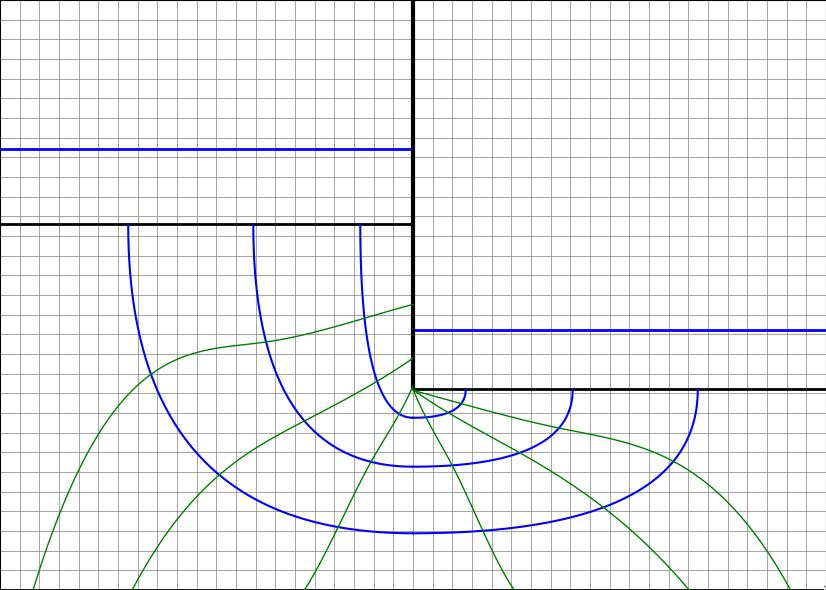
\includegraphics[width=\textwidth]{FOTOS/caso_1dibujo_base.jpg}
      \caption{Caso 1 Base}
  \end{minipage}
  \begin{minipage}{0.32\textwidth}
      \centering
      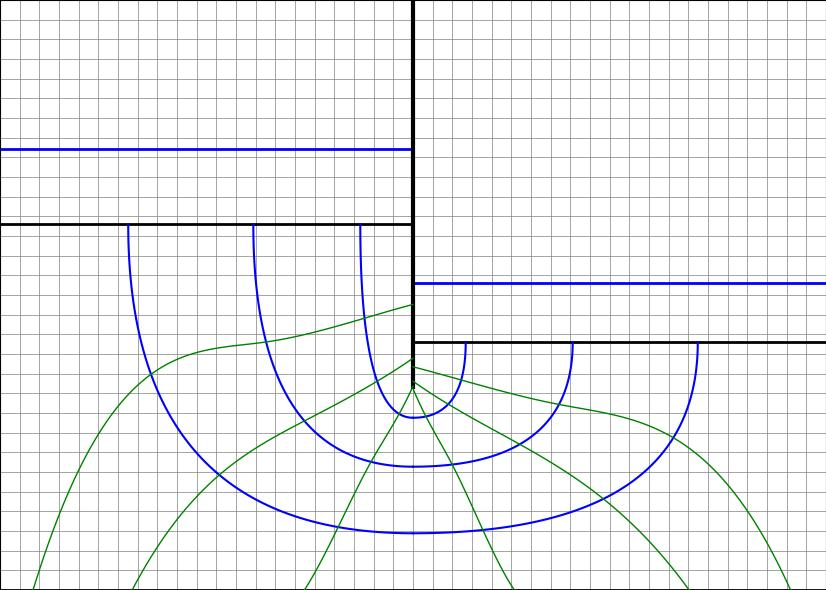
\includegraphics[width=\textwidth]{FOTOS/caso_2dibujo_base.jpg}
      \caption{Caso 2 Base}
  \end{minipage}
  \begin{minipage}{0.32\textwidth}
      \centering
      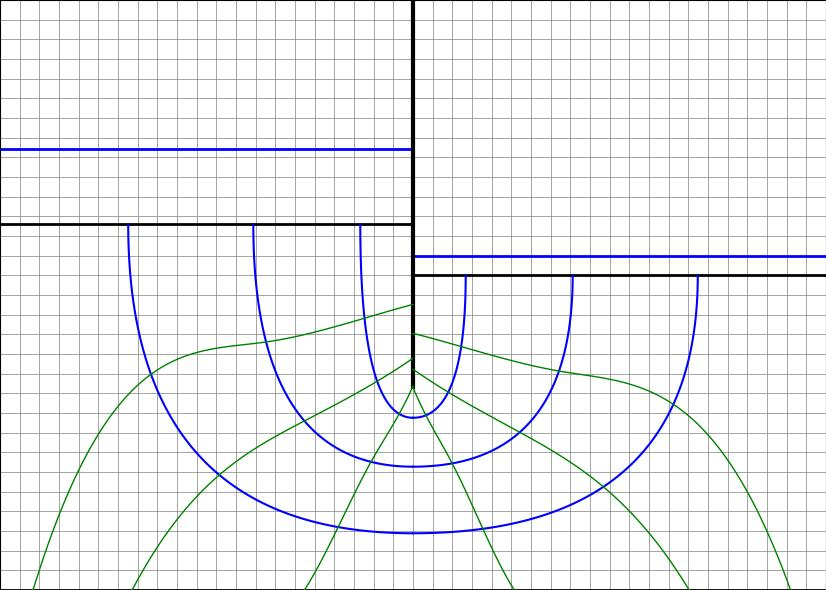
\includegraphics[width=\textwidth]{FOTOS/caso_3dibujo_base.jpg}
      \caption{Caso 3 Base}
  \end{minipage}
\end{figure}

Los dibujos en tamaño A4 como fue solicitado, y con un espaciado de 5mm (en escala correspondiente a 1 metro), se encunetran en
el siguiente link: \href{https://github.com/LukasWolff2002/PROYECTO_1_MCOCo}{Dibujos A4}.

\subsection{Presion de Poros}

\subsection{Presion Ataguia}

\subsubsection{Presiones Totales}

\begin{figure}[H]
  \centering
  \begin{minipage}{0.32\textwidth}
      \centering
      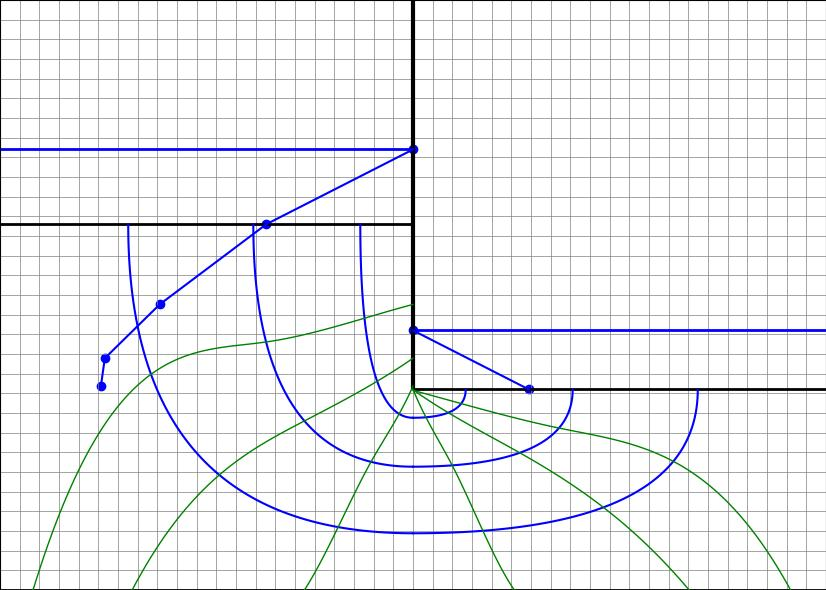
\includegraphics[width=\textwidth]{FOTOS/caso_1_presion_ataquia_total.jpg}
      \caption{Caso 1 Presiones Ataguia}
  \end{minipage}
  \begin{minipage}{0.32\textwidth}
      \centering
      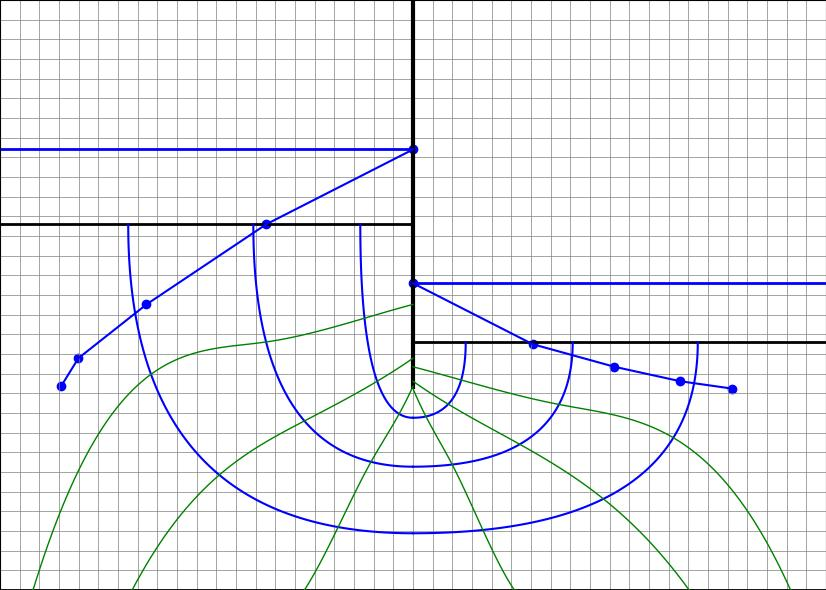
\includegraphics[width=\textwidth]{FOTOS/caso_2_presion_ataquia_total.jpg}
      \caption{Caso 2 Presiones Ataguia}
  \end{minipage}
  \begin{minipage}{0.32\textwidth}
      \centering
      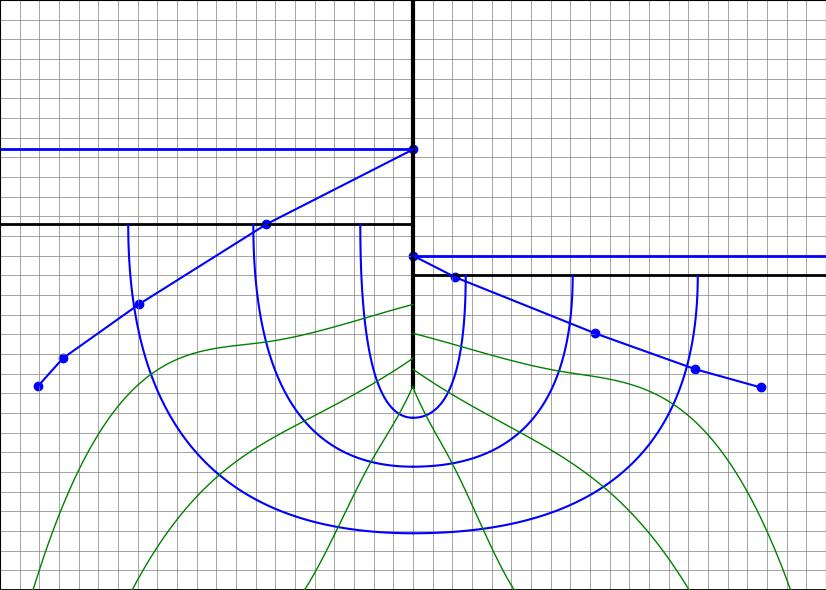
\includegraphics[width=\textwidth]{FOTOS/caso_3_presion_ataquia_total.jpg}
      \caption{Caso 3 Presiones Ataguia}
  \end{minipage}
\end{figure}

Donde las presiones en los distintos puntos solicitados son:

\begin{table}[H]
  \centering
  \begin{tabular}{|c|c|c|c|c|c|c|c|c|}
    \hline
    Caso & A & B & C & D & E & F & G & H \\
    \hline
    1 & 0 & 37.28 & 71.14 & 79.33 & 79.35 & 68.13 & 63.59 & 0 \\ \hline
    2 & 0 & 37.28 & 59.70 & 78.65 & 89.44 & 81.17 & 27.47 & 0 \\ \hline
    3 & 0 & 37.28 & 50.01 & 56.37 & 95.33 & 88.45 & 7.85 & 0 \\
    \hline
  \end{tabular}
  \caption{Presiones en Ataguia en [KPa]}
\end{table}


Para calcular esta presiones, se primero se calcularon las presiones en los distintos puntos conocidos de las lineas piezometircas:

\begin{lstlisting}[language=Python]
  #Primero Calulo el delta H, el cual debe ser en metros
  Delta_H = (C1+B1) - (C2+B2)

  #Luego calculo Z, el cual es la altura para el grafico obtenido
  #a partir de una lista de coordenadas, por lo tanto, 
  #conviero las coordenas a metros.
  z = ((coor[clave][1]-altura_rel)*200)/1000

  #Calculo Zg
  Zg = z

  #Luego calculo ni, el numero de linea equipotencial
  ni = int(clave.split('_')[1])

  #en base a esto, es posible obtener delta_hi
  Delta_Hi = (C1+B1)-((Delta_H*ni)/Nd)

  #Calculo hp
  hp = Delta_Hi-Zg

  #Y finalmente U en [KPa]
  u = (hp*gamma_agua)/1000
  
  #Este proceso es aplicado en todos los puntos conocidos
  
\end{lstlisting}

Posteriormente, aplico una regrecion lineal a la curva obtenida y asi calculo las presiones en los distintos puntos solicitados.

\begin{lstlisting}[language=Python]
  from scipy.interpolate import interp1d

  interpolacion = interp1d(x_known, y_known, kind='linear')
\end{lstlisting}

En base a todas las presiones de poros conocidas, fue posible aplicar un mapa de calor:

\subsubsection{Mapa de Presion}

\begin{figure}[H]
  \centering
  \begin{minipage}{0.32\textwidth}
      \centering
      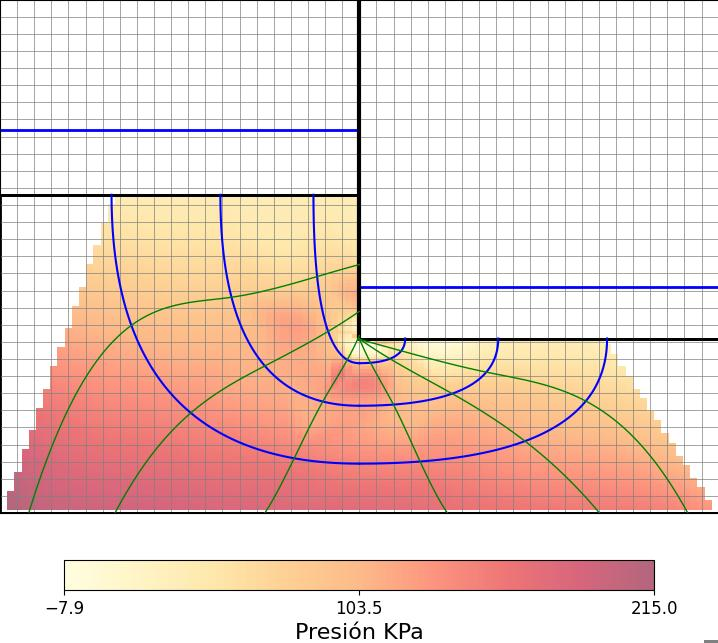
\includegraphics[width=\textwidth]{FOTOS/caso_1_mapa_calor.jpg}
      \caption{Caso 1 Presiones de Poros}
  \end{minipage}
  \begin{minipage}{0.32\textwidth}
      \centering
      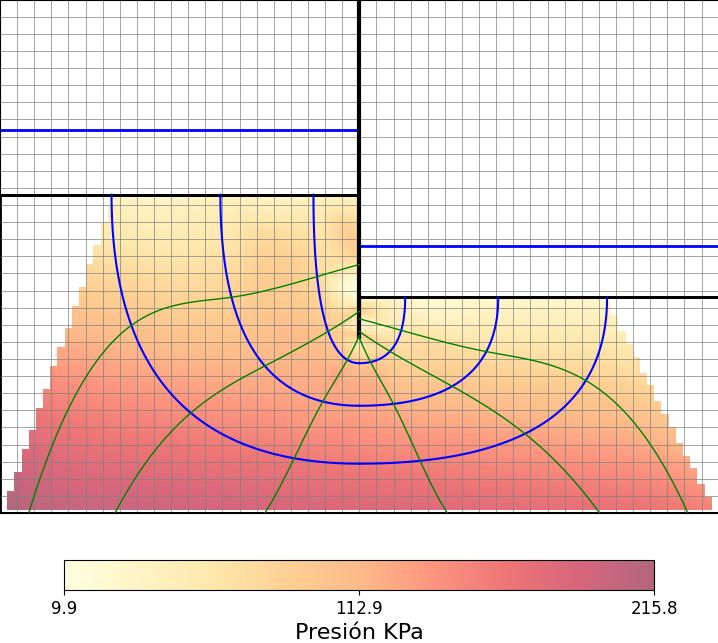
\includegraphics[width=\textwidth]{FOTOS/caso_2_mapa_calor.jpg}
      \caption{Caso 2 Presiones de Poros}
  \end{minipage}
  \begin{minipage}{0.32\textwidth}
      \centering
      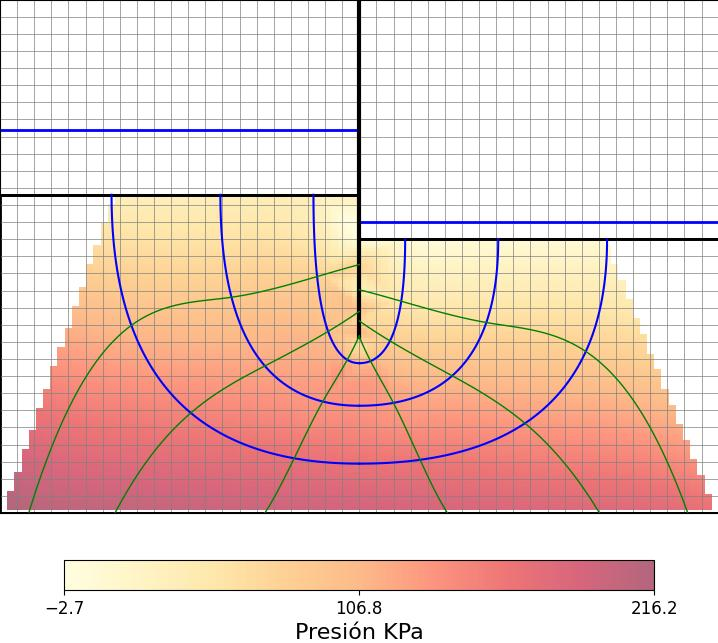
\includegraphics[width=\textwidth]{FOTOS/caso_3_mapa_calor.jpg}
      \caption{Caso 3 Presiones de Poros}
  \end{minipage}
\end{figure}

\subsubsection{Presiones Netas}

\begin{figure}[H]
  \centering
  \begin{minipage}{0.32\textwidth}
      \centering
      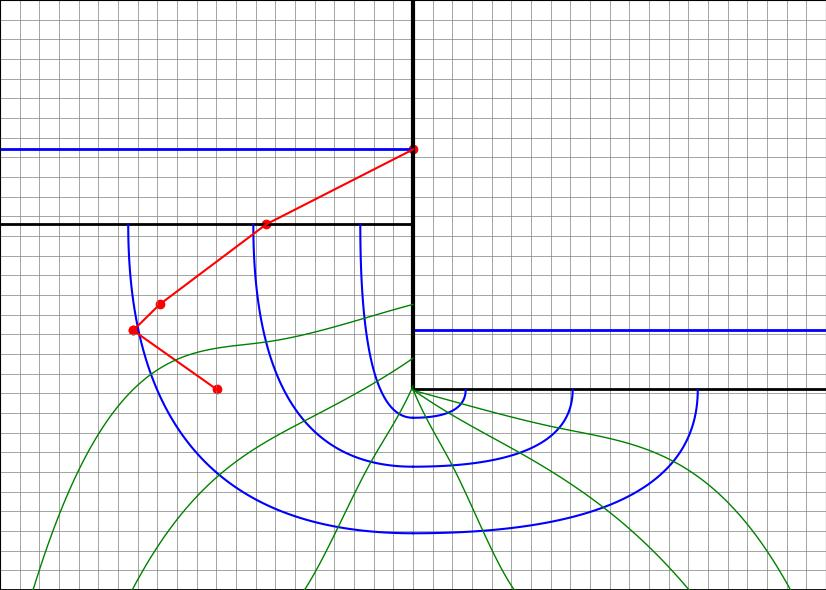
\includegraphics[width=\textwidth]{FOTOS/caso_1_presion_ataquia_neta.jpg}
      \caption{Caso 1 Presiones Ataguia Neta}
  \end{minipage}
  \begin{minipage}{0.32\textwidth}
      \centering
      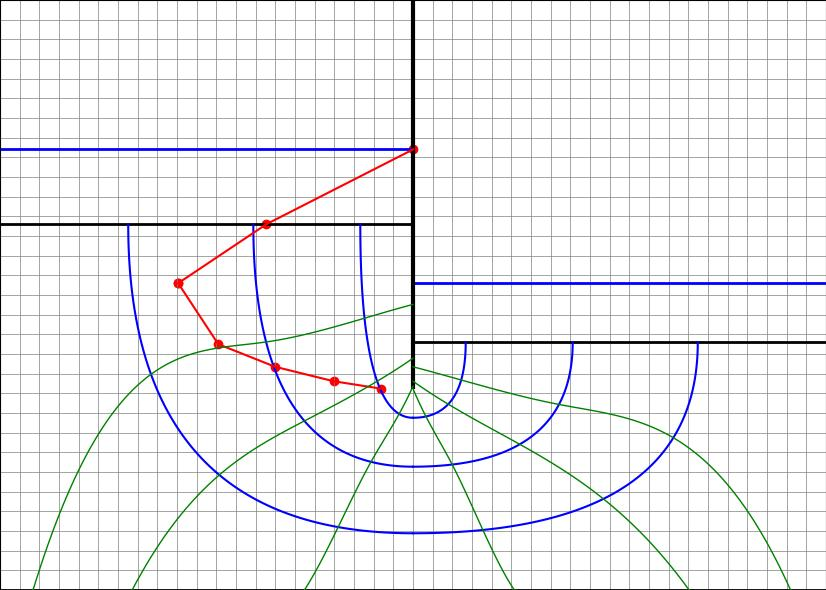
\includegraphics[width=\textwidth]{FOTOS/caso_2_presion_ataquia_neta.jpg}
      \caption{Caso 2 Presiones Ataguia Neta}
  \end{minipage}
  \begin{minipage}{0.32\textwidth}
      \centering
      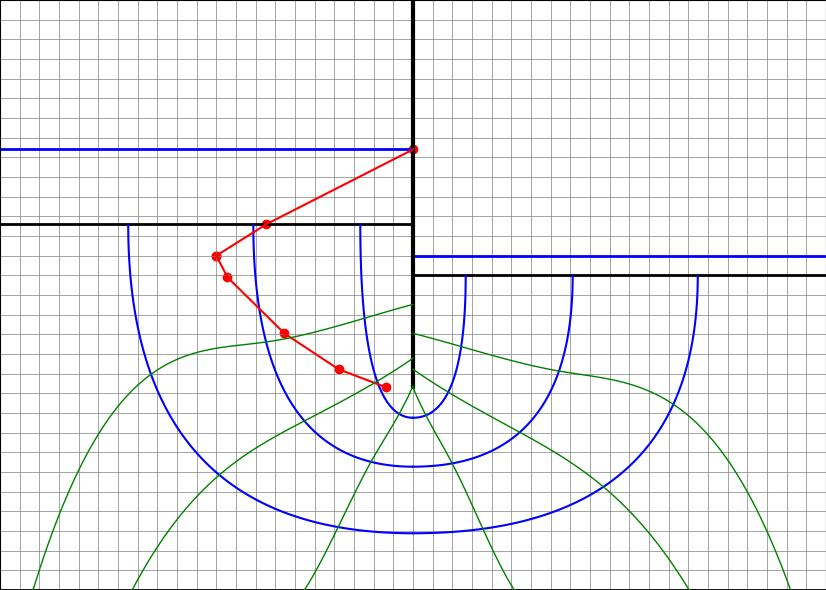
\includegraphics[width=\textwidth]{FOTOS/caso_3_presion_ataquia_neta.jpg}
      \caption{Caso 3 Presiones Ataguia Neta}
  \end{minipage}
\end{figure}

De lo cual es posible conocer el equilibrio estatico de la ataguia:

\subsubsection{Centroide de la distribucion de Presiones}

La siguiente funcion en python permite conocer el centroide de una funcion:

\begin{lstlisting}[language=Python]
  import numpy as np
  from scipy.integrate import simps

  # Calcular el area bajo la curva usando integracion numerica (Simpson)
  area = simps(y, x)

  # Centroide en x
  x_bar = simps(x * y, x) / area
  
\end{lstlisting}

De lo cual se obtiene lo siguiente:

\begin{figure}[H]
  \centering
  \begin{minipage}{0.32\textwidth}
      \centering
      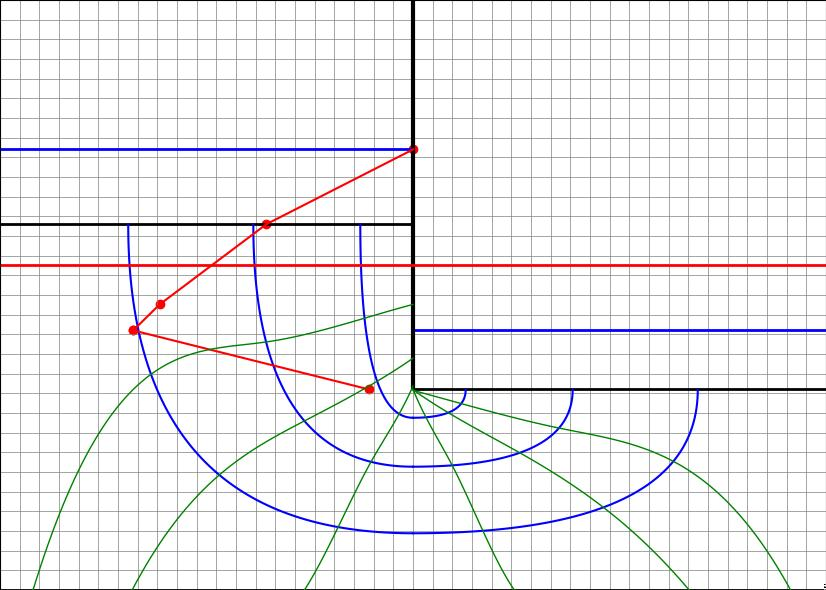
\includegraphics[width=\textwidth]{FOTOS/caso_1_centroide_y.jpg}
      \caption{Caso 1 Centroide Presiones}
  \end{minipage}
  \begin{minipage}{0.32\textwidth}
      \centering
      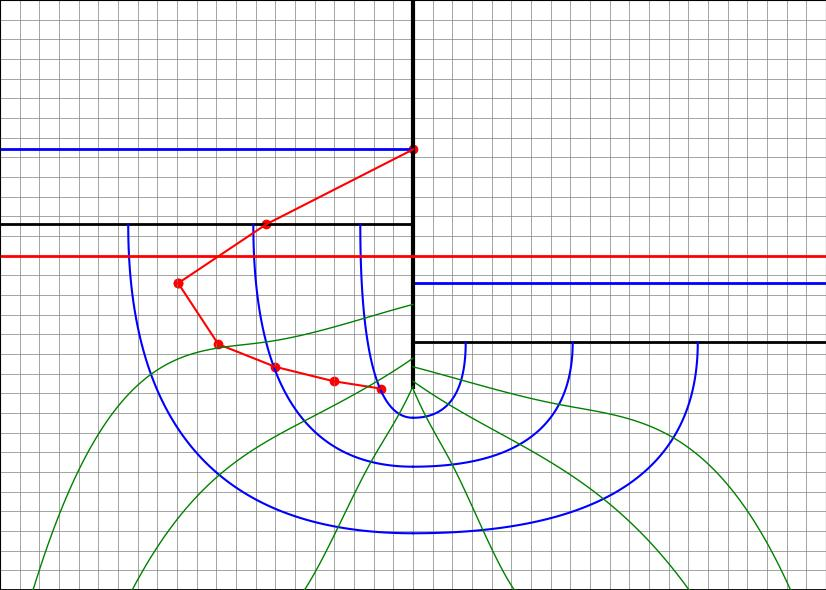
\includegraphics[width=\textwidth]{FOTOS/caso_2_centroide_y.jpg}
      \caption{Caso 2 Centroide Presiones}
  \end{minipage}
  \begin{minipage}{0.32\textwidth}
      \centering
      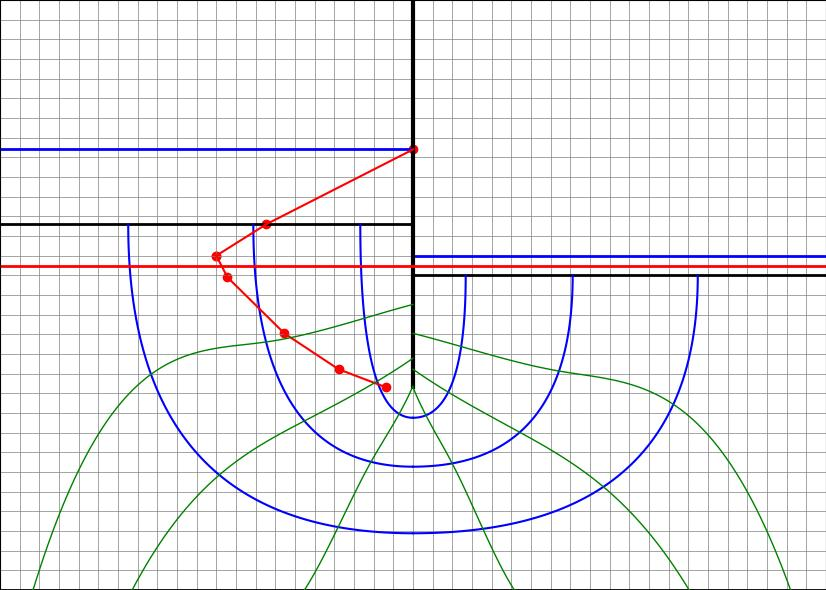
\includegraphics[width=\textwidth]{FOTOS/caso_3_centroide_y.jpg}
      \caption{Caso 3 Centroide Presiones}
  \end{minipage}
\end{figure}

\subsection{Maximo Gradiente Hidraulico}

Se calculo el maximo gradiente hidraulico como:

\begin{lstlisting}[language=Python]
  max_g = Delta_H/((C1-C2) + 2*D)
  #es decir, el minimo recorrido posible entre los dos puntos
  #Donde delta_H ya fue definido anteriormente
\end{lstlisting}

De lo cual se obtuvo:

\begin{table}[H]
  \centering
  \begin{tabular}{|c|c|c|c|}
    \hline
    Caso & Maximo Gradiente Hidraulico \\
    \hline
    1 & 1.095 \\ \hline
    2 & 0.629 \\ \hline
    3 & 0.380 \\
    \hline
  \end{tabular}
  \caption{Maximo Gradiente Hidraulico}
\end{table}

\subsection{Falla por Licuefaccion}

Definir que es la Licuefaccion

\subsection{Factor de Seguridad}

hola

\end{document}
